\documentclass[twoside]{book}

% Packages required by doxygen
\usepackage{fixltx2e}
\usepackage{calc}
\usepackage{doxygen}
\usepackage[export]{adjustbox} % also loads graphicx
\usepackage{graphicx}
\usepackage[utf8]{inputenc}
\usepackage{makeidx}
\usepackage{multicol}
\usepackage{multirow}
\PassOptionsToPackage{warn}{textcomp}
\usepackage{textcomp}
\usepackage[nointegrals]{wasysym}
\usepackage[table]{xcolor}

% Font selection
\usepackage[T1]{fontenc}
\usepackage[scaled=.90]{helvet}
\usepackage{courier}
\usepackage{amssymb}
\usepackage{sectsty}
\renewcommand{\familydefault}{\sfdefault}
\allsectionsfont{%
  \fontseries{bc}\selectfont%
  \color{darkgray}%
}
\renewcommand{\DoxyLabelFont}{%
  \fontseries{bc}\selectfont%
  \color{darkgray}%
}
\newcommand{\+}{\discretionary{\mbox{\scriptsize$\hookleftarrow$}}{}{}}

% Page & text layout
\usepackage{geometry}
\geometry{%
  a4paper,%
  top=2.5cm,%
  bottom=2.5cm,%
  left=2.5cm,%
  right=2.5cm%
}
\tolerance=750
\hfuzz=15pt
\hbadness=750
\setlength{\emergencystretch}{15pt}
\setlength{\parindent}{0cm}
\setlength{\parskip}{3ex plus 2ex minus 2ex}
\makeatletter
\renewcommand{\paragraph}{%
  \@startsection{paragraph}{4}{0ex}{-1.0ex}{1.0ex}{%
    \normalfont\normalsize\bfseries\SS@parafont%
  }%
}
\renewcommand{\subparagraph}{%
  \@startsection{subparagraph}{5}{0ex}{-1.0ex}{1.0ex}{%
    \normalfont\normalsize\bfseries\SS@subparafont%
  }%
}
\makeatother

% Headers & footers
\usepackage{fancyhdr}
\pagestyle{fancyplain}
\fancyhead[LE]{\fancyplain{}{\bfseries\thepage}}
\fancyhead[CE]{\fancyplain{}{}}
\fancyhead[RE]{\fancyplain{}{\bfseries\leftmark}}
\fancyhead[LO]{\fancyplain{}{\bfseries\rightmark}}
\fancyhead[CO]{\fancyplain{}{}}
\fancyhead[RO]{\fancyplain{}{\bfseries\thepage}}
\fancyfoot[LE]{\fancyplain{}{}}
\fancyfoot[CE]{\fancyplain{}{}}
\fancyfoot[RE]{\fancyplain{}{\bfseries\scriptsize Generated by Doxygen }}
\fancyfoot[LO]{\fancyplain{}{\bfseries\scriptsize Generated by Doxygen }}
\fancyfoot[CO]{\fancyplain{}{}}
\fancyfoot[RO]{\fancyplain{}{}}
\renewcommand{\footrulewidth}{0.4pt}
\renewcommand{\chaptermark}[1]{%
  \markboth{#1}{}%
}
\renewcommand{\sectionmark}[1]{%
  \markright{\thesection\ #1}%
}

% Indices & bibliography
\usepackage{natbib}
\usepackage[titles]{tocloft}
\setcounter{tocdepth}{3}
\setcounter{secnumdepth}{5}
\makeindex

% Hyperlinks (required, but should be loaded last)
\usepackage{ifpdf}
\ifpdf
  \usepackage[pdftex,pagebackref=true]{hyperref}
\else
  \usepackage[ps2pdf,pagebackref=true]{hyperref}
\fi
\hypersetup{%
  colorlinks=true,%
  linkcolor=blue,%
  citecolor=blue,%
  unicode%
}

% Custom commands
\newcommand{\clearemptydoublepage}{%
  \newpage{\pagestyle{empty}\cleardoublepage}%
}

\usepackage{caption}
\captionsetup{labelsep=space,justification=centering,font={bf},singlelinecheck=off,skip=4pt,position=top}

%===== C O N T E N T S =====

\begin{document}

% Titlepage & ToC
\hypersetup{pageanchor=false,
             bookmarksnumbered=true,
             pdfencoding=unicode
            }
\pagenumbering{alph}
\begin{titlepage}
\vspace*{7cm}
\begin{center}%
{\Large My Project }\\
\vspace*{1cm}
{\large Generated by Doxygen 1.8.14}\\
\end{center}
\end{titlepage}
\clearemptydoublepage
\pagenumbering{roman}
\tableofcontents
\clearemptydoublepage
\pagenumbering{arabic}
\hypersetup{pageanchor=true}

%--- Begin generated contents ---
\chapter{Module Index}
\section{Modules}
Here is a list of all modules\+:\begin{DoxyCompactList}
\item \contentsline{section}{Srook\+\_\+math\+\_\+primes\+\_\+counting}{\pageref{group__srook__math__primes__counting}}{}
\item \contentsline{section}{Srook\+\_\+math\+\_\+primes\+\_\+progression}{\pageref{group__srook__math__primes__progression}}{}
\end{DoxyCompactList}

\chapter{Class Index}
\section{Class List}
Here are the classes, structs, unions and interfaces with brief descriptions\+:\begin{DoxyCompactList}
\item\contentsline{section}{\mbox{\hyperlink{structlegendre}{legendre}} }{\pageref{structlegendre}}{}
\item\contentsline{section}{\mbox{\hyperlink{classsieve__atkin}{sieve\+\_\+atkin}} }{\pageref{classsieve__atkin}}{}
\item\contentsline{section}{\mbox{\hyperlink{classsieve__eratosthenese}{sieve\+\_\+eratosthenese}} }{\pageref{classsieve__eratosthenese}}{}
\item\contentsline{section}{\mbox{\hyperlink{classsieve__euler}{sieve\+\_\+euler}} \\*Global namespace srook }{\pageref{classsieve__euler}}{}
\item\contentsline{section}{\mbox{\hyperlink{classsieve__sundaram}{sieve\+\_\+sundaram}} }{\pageref{classsieve__sundaram}}{}
\end{DoxyCompactList}

\chapter{File Index}
\section{File List}
Here is a list of all documented files with brief descriptions\+:\begin{DoxyCompactList}
\item\contentsline{section}{{\bfseries counting.\+hpp} }{\pageref{counting_8hpp}}{}
\item\contentsline{section}{{\bfseries progression.\+hpp} }{\pageref{progression_8hpp}}{}
\item\contentsline{section}{counting/\mbox{\hyperlink{legendre_8hpp}{legendre.\+hpp}} \\*The prime number counting function by Legendre (1808) }{\pageref{legendre_8hpp}}{}
\item\contentsline{section}{counting/{\bfseries sieve\+\_\+atkin.\+hpp} }{\pageref{counting_2sieve__atkin_8hpp}}{}
\item\contentsline{section}{counting/{\bfseries sieve\+\_\+eratosthenese.\+hpp} }{\pageref{counting_2sieve__eratosthenese_8hpp}}{}
\item\contentsline{section}{counting/{\bfseries sieve\+\_\+euler.\+hpp} }{\pageref{counting_2sieve__euler_8hpp}}{}
\item\contentsline{section}{counting/{\bfseries sieve\+\_\+sundaram.\+hpp} }{\pageref{counting_2sieve__sundaram_8hpp}}{}
\item\contentsline{section}{progression/{\bfseries sieve\+\_\+atkin.\+hpp} }{\pageref{progression_2sieve__atkin_8hpp}}{}
\item\contentsline{section}{progression/{\bfseries sieve\+\_\+eratosthenese.\+hpp} }{\pageref{progression_2sieve__eratosthenese_8hpp}}{}
\item\contentsline{section}{progression/{\bfseries sieve\+\_\+euler.\+hpp} }{\pageref{progression_2sieve__euler_8hpp}}{}
\item\contentsline{section}{progression/{\bfseries sieve\+\_\+sundaram.\+hpp} }{\pageref{progression_2sieve__sundaram_8hpp}}{}
\end{DoxyCompactList}

\chapter{Module Documentation}
\hypertarget{group__srook__math__primes__counting}{}\section{Srook\+\_\+math\+\_\+primes\+\_\+counting}
\label{group__srook__math__primes__counting}\index{Srook\+\_\+math\+\_\+primes\+\_\+counting@{Srook\+\_\+math\+\_\+primes\+\_\+counting}}
Collaboration diagram for Srook\+\_\+math\+\_\+primes\+\_\+counting\+:\nopagebreak
\begin{figure}[H]
\begin{center}
\leavevmode
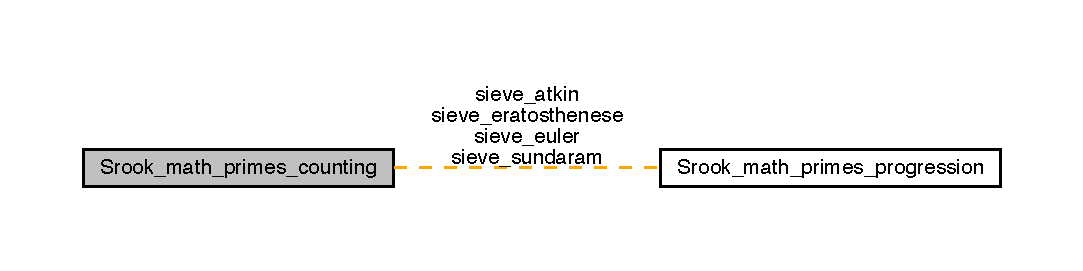
\includegraphics[width=350pt]{group__srook__math__primes__counting}
\end{center}
\end{figure}
\subsection*{Classes}
\begin{DoxyCompactItemize}
\item 
struct \mbox{\hyperlink{structlegendre}{legendre}}
\item 
class \mbox{\hyperlink{classsieve__atkin}{sieve\+\_\+atkin}}
\item 
class \mbox{\hyperlink{classsieve__eratosthenese}{sieve\+\_\+eratosthenese}}
\item 
class \mbox{\hyperlink{classsieve__euler}{sieve\+\_\+euler}}
\begin{DoxyCompactList}\small\item\em global namespace srook \end{DoxyCompactList}\item 
class \mbox{\hyperlink{classsieve__sundaram}{sieve\+\_\+sundaram}}
\end{DoxyCompactItemize}


\subsection{Detailed Description}

\hypertarget{group__srook__math__primes__progression}{}\section{Srook\+\_\+math\+\_\+primes\+\_\+progression}
\label{group__srook__math__primes__progression}\index{Srook\+\_\+math\+\_\+primes\+\_\+progression@{Srook\+\_\+math\+\_\+primes\+\_\+progression}}
Collaboration diagram for Srook\+\_\+math\+\_\+primes\+\_\+progression\+:\nopagebreak
\begin{figure}[H]
\begin{center}
\leavevmode
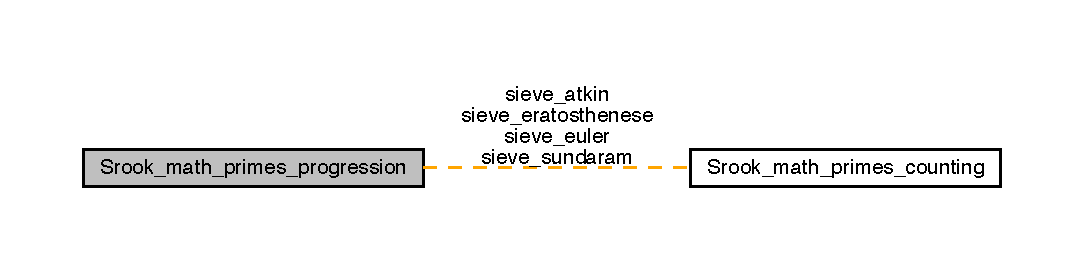
\includegraphics[width=350pt]{group__srook__math__primes__progression}
\end{center}
\end{figure}
\subsection*{Classes}
\begin{DoxyCompactItemize}
\item 
class \mbox{\hyperlink{classsieve__atkin}{sieve\+\_\+atkin}}
\item 
class \mbox{\hyperlink{classsieve__eratosthenese}{sieve\+\_\+eratosthenese}}
\item 
class \mbox{\hyperlink{classsieve__euler}{sieve\+\_\+euler}}
\begin{DoxyCompactList}\small\item\em global namespace srook \end{DoxyCompactList}\item 
class \mbox{\hyperlink{classsieve__sundaram}{sieve\+\_\+sundaram}}
\end{DoxyCompactItemize}


\subsection{Detailed Description}

\chapter{Class Documentation}
\hypertarget{structlegendre}{}\section{legendre Struct Reference}
\label{structlegendre}\index{legendre@{legendre}}


The documentation for this struct was generated from the following file\+:\begin{DoxyCompactItemize}
\item 
counting/\mbox{\hyperlink{legendre_8hpp}{legendre.\+hpp}}\end{DoxyCompactItemize}

\hypertarget{classsieve__atkin}{}\section{sieve\+\_\+atkin Class Reference}
\label{classsieve__atkin}\index{sieve\+\_\+atkin@{sieve\+\_\+atkin}}


The documentation for this class was generated from the following file\+:\begin{DoxyCompactItemize}
\item 
counting/sieve\+\_\+atkin.\+hpp\end{DoxyCompactItemize}

\hypertarget{classsieve__eratosthenese}{}\section{sieve\+\_\+eratosthenese Class Reference}
\label{classsieve__eratosthenese}\index{sieve\+\_\+eratosthenese@{sieve\+\_\+eratosthenese}}


The documentation for this class was generated from the following file\+:\begin{DoxyCompactItemize}
\item 
counting/sieve\+\_\+eratosthenese.\+hpp\end{DoxyCompactItemize}

\hypertarget{classsieve__euler}{}\section{sieve\+\_\+euler Class Reference}
\label{classsieve__euler}\index{sieve\+\_\+euler@{sieve\+\_\+euler}}


global namespace srook  




{\ttfamily \#include $<$sieve\+\_\+euler.\+hpp$>$}



\subsection{Detailed Description}
global namespace srook 

The documentation for this class was generated from the following file\+:\begin{DoxyCompactItemize}
\item 
counting/sieve\+\_\+euler.\+hpp\end{DoxyCompactItemize}

\hypertarget{classsieve__sundaram}{}\section{sieve\+\_\+sundaram Class Reference}
\label{classsieve__sundaram}\index{sieve\+\_\+sundaram@{sieve\+\_\+sundaram}}


The documentation for this class was generated from the following file\+:\begin{DoxyCompactItemize}
\item 
counting/sieve\+\_\+sundaram.\+hpp\end{DoxyCompactItemize}

\chapter{File Documentation}
\hypertarget{legendre_8hpp}{}\section{counting/legendre.hpp File Reference}
\label{legendre_8hpp}\index{counting/legendre.\+hpp@{counting/legendre.\+hpp}}


The prime number counting function by Legendre (1808)  


{\ttfamily \#include $<$srook/config.\+hpp$>$}\newline
{\ttfamily \#include $<$srook/type\+\_\+traits/is\+\_\+integral.\+hpp$>$}\newline
{\ttfamily \#include $<$srook/type\+\_\+traits/enable\+\_\+if.\+hpp$>$}\newline
{\ttfamily \#include $<$srook/math/constants/algorithm/log.\+hpp$>$}\newline
Include dependency graph for legendre.\+hpp\+:\nopagebreak
\begin{figure}[H]
\begin{center}
\leavevmode
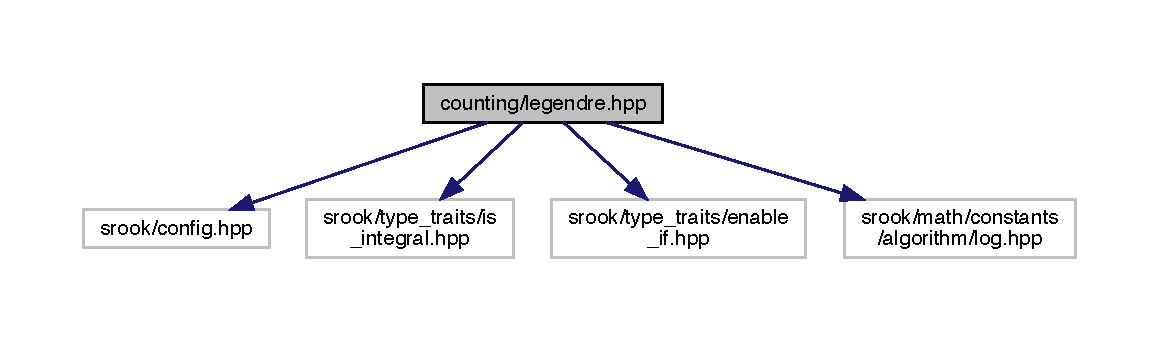
\includegraphics[width=350pt]{legendre_8hpp__incl}
\end{center}
\end{figure}
This graph shows which files directly or indirectly include this file\+:\nopagebreak
\begin{figure}[H]
\begin{center}
\leavevmode
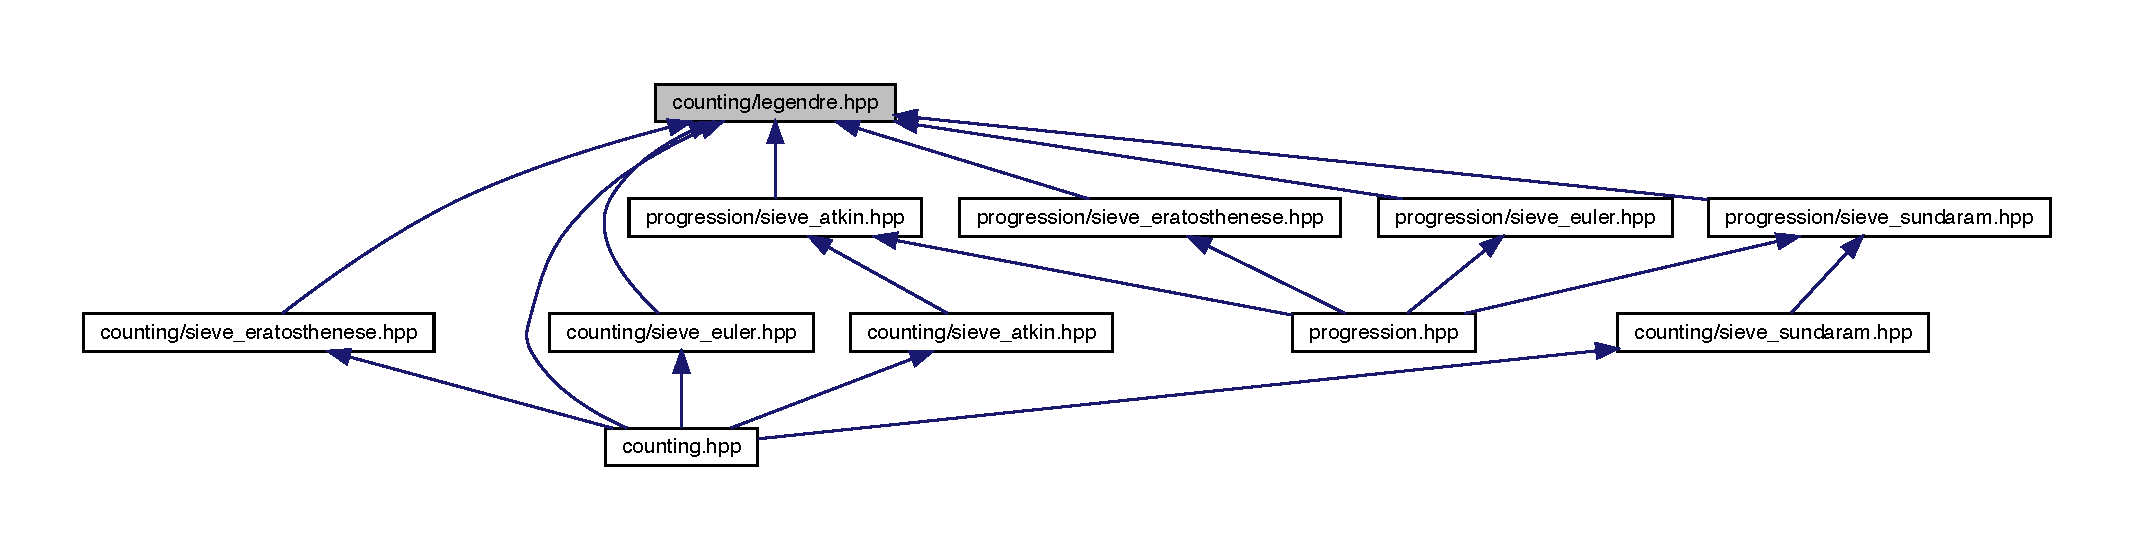
\includegraphics[width=350pt]{legendre_8hpp__dep__incl}
\end{center}
\end{figure}


\subsection{Detailed Description}
The prime number counting function by Legendre (1808) 

\begin{DoxyAuthor}{Author}
roki 
\end{DoxyAuthor}
\begin{DoxyParagraph}{Copyright}
Copyright (C) 2011-\/2018 Roki. Distributed under the M\+IT License. 
\end{DoxyParagraph}

%--- End generated contents ---

% Index
\backmatter
\newpage
\phantomsection
\clearemptydoublepage
\addcontentsline{toc}{chapter}{Index}
\printindex

\end{document}
